\subsection{General Statements about Homology}

In the following let $(H_\bullet,\partial_\bullet)$ be any homology theory.

\begin{lemma}
    Let $A \subseteq X$ be a retract. Then $H_\bullet(X) \cong H_\bullet(X,A) \oplus H_\bullet(A)$.
\end{lemma}

\begin{proof}
    Let $r \colon X \to A$ be a retraction and $i \colon A \to X$ the inclusion. Then $H_\bullet(r) \circ H_\bullet(i) = \mathrm{id}_{H_\bullet(A)}$, in particular $H_\bullet(i)$ is injective. Hence the long exact sequence for the pair $(X,A)$ breaks up into short split exact sequences
    \begin{center}
        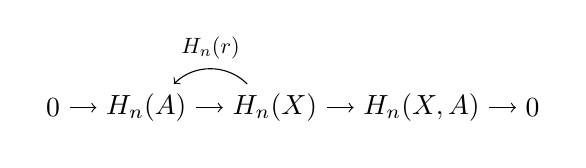
\begin{tikzpicture}
            \matrix[column sep = 10pt, row sep =15pt]
            {
                \node (zero1) {$0$}; &
                \node (hna) {$H_n(A)$}; &
                \node (hnx) {$H_n(X)$}; &
                \node (hnxa) {$H_n(X,A)$}; &
                \node (zero2) {$0$}; \\
            };

            \draw[->] (zero1.east) -- (hna.west);
            \draw[->] (hna.east) -- (hnx.west);
            \draw[->] (hnx.east) -- (hnxa.west);
            \draw[->] (hnxa.east) -- (zero2.west);
            \draw[->, bend right=45] ([xshift=-10pt]hnx.north) to node[above] {\scalebox{0.8}{$H_n(r)$}} ([xshift=10pt]hna.north);
        \end{tikzpicture}
    \end{center}
    and the splitting lemma yields the desired isomorphism.
\end{proof}

\begin{lemma}
    Let $f \colon (X,A) \to (Y,B)$ be a continuous map of pairs, such that $f \colon X \to Y$ and $f \colon A \to B$ are homotopy equivalences. Then $f$ induces an isomorphism
    \[
    H_\bullet(f) \colon H_\bullet(X,A) \to H_\bullet(Y,B).
    \] 
\end{lemma}

\begin{remark}
    Note that $f \colon (X,A) \to (Y,B)$ is not necessarily a homotopy equivalence of \textit{pairs}. See chapter 3 in \cite{steimle_alg_topo} for a counterexample.
\end{remark}

\begin{proof}
    Consider the map between the long exact sequences of the pairs $(X,A)$ and $(Y,B)$ induced by $f$: 
    \[\begin{tikzcd}[column sep = 1.3em]
	\cdots & {H_n(A)} & {H_n(X)} & {H_n(X,A)} & {H_{n-1}(A)} & {H_{n-1}(X)} & \cdots \\
	\cdots & {H_n(B)} & {H_n(Y)} & {H_n(Y,B)} & {H_{n-1}(B)} & {H_{n-1}(Y)} & \cdots
	\arrow[from=1-1, to=1-2]
	\arrow[from=1-2, to=1-3]
	\arrow["{H_n(f)}", "\cong"', from=1-2, to=2-2]
	\arrow[from=1-3, to=1-4]
	\arrow["{H_n(f)}", "\cong"', from=1-3, to=2-3]
	\arrow[from=1-4, to=1-5]
	\arrow["{H_n(f)}", from=1-4, to=2-4]
	\arrow[from=1-5, to=1-6]
	\arrow["{H_{n-1}(f)}", "\cong"', from=1-5, to=2-5]
	\arrow[from=1-6, to=1-7]
	\arrow["{H_{n-1}(f)}", "\cong"', from=1-6, to=2-6]
	\arrow[from=2-1, to=2-2]
	\arrow[from=2-2, to=2-3]
	\arrow[from=2-3, to=2-4]
	\arrow[from=2-4, to=2-5]
	\arrow[from=2-5, to=2-6]
	\arrow[from=2-6, to=2-7]
\end{tikzcd}\]
The outer maps are isomorphisms by homotopy invariance and so the five lemma implies that the middle map is an isomorphism as well.
\end{proof}

\begin{lemma}
    Let $A \subseteq X$ be a closed neighbourhood-deformation retract. Then the projection $X \to X/A$ induces a natural isomorphism $$H_\bullet(X,A) \to H_\bullet(X/A,\ast).$$
\end{lemma}
\begin{proof}
    Applying excision in the push-out
    \begin{center}
        \commsquare{$A$}{$X$}{$\ast$}{$X/A$}{}{}{}{}
    \end{center}
    shows that the projection induces an isomorphism. Furthermore, any map $(X,A) \to (Y,B)$ descends to a map $X/A \to Y/B$ and naturality then just follows from functoriality. 
\end{proof}

\begin{definition}
    Let $(H_\bullet,\partial_\bullet)$ and $(H_\bullet^\prime,\partial_\bullet^\prime)$ be homology theories with values in $R$-$\mathsf{Mod}$. A natural transformation of homology theories is a natural transformation $\eta \colon H_\bullet \to H_\bullet^\prime$ of functors, which is compatible with the boundary maps, that is $\eta \circ \partial_\bullet = \partial_\bullet^\prime \circ \eta$. Similiarly we define a natural transformation of cohomology theories.
\end{definition}

For singular (co)homology the so called \textbf{change of coefficients homomorphism} introduced in the following Proposition is a natural transformation of (co)homology theories.

\begin{proposition}
    Let $M$ and $N$ be $R$-Modules and $\phi \colon M \to N$ an $R$-linear map. Then $\phi$ induces a natural transformation 
    \[
    \eta(\phi) \colon (H_\bullet^\mathrm{sing}(-;M),\partial_\bullet) \to (H_\bullet^\mathrm{sing}(-;N),\partial_\bullet)
    \]
    of homology theories called the \textbf{change of coefficients homomorphism}. Moreover the assignment $\phi \mapsto \eta(\phi)$ is functorial, such that we get a functor from $R$-$\mathsf{Mod}$ into the category of homology theories with values in $R$-$\mathsf{Mod}$. Similiarly $\phi$ induces a natural transformation 
    \[
    \delta(\phi) \colon (H^\bullet_\mathrm{sing}(-;M),\partial^\bullet) \to (H^\bullet_\mathrm{sing}(-;N),\partial^\bullet)
    \]
    of cohomology theories. Again the assignment $\phi \mapsto \delta(\phi)$ is functorial.
\end{proposition}

\begin{proof}
    Let $(X,B,A)$ be a triple of topological spaces. Define 
    \[
    \eta_{\mathsf{Ch}}(\phi) \colon C_\bullet^\mathrm{sing}(X;M) \to C_\bullet^\mathrm{sing}(X;N)
    \]
    by 
    \[
    \sum_{\sigma \in \mathrm{Sing}_n(X)} \hspace{-1em} m_\sigma \sigma \hspace{1em} \mapsto \sum_{\sigma \in \mathrm{Sing}_n(X)} \hspace{-1em} \phi(m_\sigma) \sigma.
    \]
    This is clearly natural in $X$ and so in particular $\eta_{\mathsf{Ch}}(\phi)$ descends to a map 
    \[
    C_\bullet^\mathrm{sing}(X,B;M) \to C_\bullet^\mathrm{sing}(X,B;N)
    \]
    of the relative chain complexes, which is again natural in $(X,A)$. Thus $\eta_{\mathsf{Ch}}(\phi)$ induces a natural transformation of functors 
    \[
    \eta(\phi) \colon H_\bullet^\mathrm{sing}(-;M) \to H_\bullet^\mathrm{sing}(-;M).
    \]
    It is also clear from the definition that $\phi \mapsto \eta(\phi)$ is functorial. To see that $\eta(\phi)$ commutes with the boundary maps note that by naturality of $\eta_{\mathsf{Ch}}(\phi)$ the following diagramm commutes 
    \[\begin{tikzcd}
	0 & {C_\bullet^\mathrm{sing}(B,A;M)} & {C_\bullet^\mathrm{sing}(X,A;M)} & {C_\bullet^\mathrm{sing}(X,B;M)} & 0 \\
	0 & {C_\bullet^\mathrm{sing}(B,A;N)} & {C_\bullet^\mathrm{sing}(X,A;N)} & {C_\bullet^\mathrm{sing}(X,B;N)} & 0
	\arrow[from=1-1, to=1-2]
	\arrow[from=1-2, to=1-3]
	\arrow[from=1-2, to=2-2]
	\arrow[from=1-3, to=1-4]
	\arrow[from=1-3, to=2-3]
	\arrow[from=1-4, to=1-5]
	\arrow[from=1-4, to=2-4]
	\arrow[from=2-1, to=2-2]
	\arrow[from=2-2, to=2-3]
	\arrow[from=2-3, to=2-4]
	\arrow[from=2-4, to=2-5]
\end{tikzcd}\]
where the horizontal maps are induced by the corresponding inclusions and the vertical maps are induced by $\eta_{\mathsf{Ch}}(\phi)$. The exact rows of this diagram induce the long exact sequences in homology, which define the boundary maps of interest. Moreover any commutative diagram of short exact sequences of this form induces a map of the long exact sequences in homology. This shows that $\eta(\phi)$ commutes with the boundary maps. 

For the statement about cohomology recall that the singular cochain complex with coefficients in $M$ is defined as 
\[
C^\bullet_\mathrm{sing}(X,B;M) := \mathrm{Hom}_R(C_\bullet^\mathrm{sing}(X,B;R),M).
\]
Thus we can simply define a natural map 
\[
\delta_\mathsf{Ch}(\phi) \colon C^\bullet_\mathrm{sing}(X,B;M) \to C^\bullet_\mathrm{sing}(X,B;N)
\]
by post-composing with $\phi$. Again the commutativity of 
\[\begin{tikzcd}
	0 & {C^\bullet_\mathrm{sing}(X,B;M)} & {C^\bullet_\mathrm{sing}(X,A;M)} & {C^\bullet_\mathrm{sing}(B,A;M)} & 0 \\
	0 & {C^\bullet_\mathrm{sing}(X,B;N)} & {C^\bullet_\mathrm{sing}(X,A;N)} & {C^\bullet_\mathrm{sing}(B,A;N)} & 0
	\arrow[from=1-1, to=1-2]
	\arrow[from=1-2, to=1-3]
	\arrow[from=1-2, to=2-2]
	\arrow[from=1-3, to=1-4]
	\arrow[from=1-3, to=2-3]
	\arrow[from=1-4, to=1-5]
	\arrow[from=1-4, to=2-4]
	\arrow[from=2-1, to=2-2]
	\arrow[from=2-2, to=2-3]
	\arrow[from=2-3, to=2-4]
	\arrow[from=2-4, to=2-5]
\end{tikzcd}\]
shows that the natural map $\delta(\phi) \colon H^\bullet_\mathrm{sing}(-;M) \to H^\bullet_\mathrm{sing}(-;N)$ induced by $\delta_\mathsf{Ch}(\phi)$ commutes with the boundary maps. The claim about functoriality also follows immediately.
\end{proof}